\documentclass[twocolumn,twoside,11pt,a4paper]{article}
\usepackage[utf8]{inputenc}     % 8 bits
\usepackage[pdftex]{graphicx}   % images .png or .pdf w/ pdflatex OR .eps w/ latex
\usepackage[T1]{fontenc}        % PS fonts
\usepackage{lmodern}            % fonts, sudo apt-get install lmodern
\usepackage{verbatim}
\usepackage{parskip}            % no indentation on paragraphs
\usepackage{tabularx}           % more on tables
\usepackage{longtable}          % more pages
\usepackage{url}                % URLs

\usepackage[sc]{mathpazo}       % Use the Palatino font
\linespread{1.05}               % Line spacing - Palatino needs more space between lines
\usepackage{microtype}          % Slightly tweak font spacing for aesthetics
\usepackage[hang, small, labelfont=bf,up,textfont=it,up]{caption} % Custom captions under/above floats in tables or figures
\usepackage{booktabs}           % Horizontal rules in tables
\usepackage{float}              % Required for tables and figures in the multi-column environment - they need to be placed in specific locations with the [H] (e.g. \begin{table}[H])
\usepackage{dblfloatfix}
\usepackage{paralist}           % Used for the compactitem environment which makes bullet points with less space between them

% geometry package
\usepackage[outer=20mm,inner=20mm,vmargin=15mm,includehead,includefoot,headheight=15pt]{geometry}
%% space between columns
\columnsep 10mm

\usepackage{abstract}           % Allows abstract customization
\renewcommand{\abstractnamefont}{\normalfont\bfseries} % Set the "Abstract" text to bold
\renewcommand{\abstracttextfont}{\normalfont\small\itshape} % Set the abstract itself to small italic text

% \usepackage{titlesec}           % Allows customization of titles
% \renewcommand\thesection{\Roman{section}} % Roman numerals for the sections
% \renewcommand\thesubsection{\Roman{subsection}} % Roman numerals for subsections
% \titleformat{\section}[block]{\large\scshape\centering}{\thesection.}{1em}{} % Change the look of the section titles
% \titleformat{\subsection}[block]{\large}{\thesubsection.}{1em}{} % Change the look of the section titles

\usepackage[pdftex]{hyperref}
\hypersetup{%
    a4paper = true,              % use A4 paper
    bookmarks = true,            % make bookmarks
    colorlinks = true,           % false: boxed links; true: colored links
    pdffitwindow = false,        % page fit to window when opened
    pdfpagemode = UseNone,       % do not show bookmarks
    pdfpagelayout = SinglePage,  % displays a single page
    pdfpagetransition = Replace, % page transition
    linkcolor=blue,              % hyperlink colors
    urlcolor=blue,
    citecolor=blue,
    anchorcolor=green
}

\usepackage{indentfirst}         % indent also 1st paragraph

\usepackage{fancyhdr}            % Headers and footers
\pagestyle{fancy}                % pages have headers and footers
\fancyhead{}                     % Blank out the default header
\fancyfoot{}                     % Blank out the default footer
\fancyhead[LO,RE]{\textit{Spotify on the rocks} - cocktails de música} % Custom header text
\fancyhead[RO,LE]{\thepage}      % Custom header text
\fancyfoot[RO,LE]{Grupo 5, \today} % Custom footer text
\renewcommand{\headrulewidth}{0.4pt}
\renewcommand{\footrulewidth}{0.4pt}

\hyphenation{}                  % explicit hyphenation

%----------------------------------------------------------------------------------------
%	macro definitions
%----------------------------------------------------------------------------------------

% entities
\newcommand{\class}[1]{{\normalfont\slshape #1\/}}
\newcommand{\svg}{\class{SVG}}
\newcommand{\scada}{\class{SCADA}}
\newcommand{\scadadms}{\class{SCADA/DMS}}

%----------------------------------------------------------------------------------------
%	TITLE SECTION
%----------------------------------------------------------------------------------------

% article title
\title{\vspace{-15mm}\fontsize{24pt}{10pt}\selectfont\textbf{Spotify on the rocks}}

% authors
\author{Ana Santos\\
\small \texttt{ansantos3@gmail.com}\\
\and
Rui Pedro Lima\\
\small \texttt{ruipedro.lima@gmail.com}
\vspace{-5mm}
}

\date{\today}

%----------------------------------------------------------------------------------------

\begin{document}

\maketitle
\thispagestyle{plain}            % no headers in the first page

%----------------------------------------------------------------------------------------
%	ABSTRACT
%----------------------------------------------------------------------------------------

\begin{abstract}


\textit{Spotify on the Rocks} é uma aplicação Web a ser desenvolvida no âmbito da unidade curricular Descrição, Armazenamento e Pesquisa de Informação (DAPI), do Mestrado Integrado em Engenharia Informática e Computação (MIEIC), da Faculdade de Engenharia da Universidade do Porto (FEUP).
A aplicação tem como principal objetivo obter grandes dimensões de informação musical, interpretá-la ao nível do input do utilizador, e representá-la de acordo com a sua componente geográfica e métrica, oferecendo ao utilizador possíveis estudos e curiosidades sobre os seus interesses musicais.

\end{abstract}

%----------------------------------------------------------------------------------------
%	ARTICLE CONTENTS
%----------------------------------------------------------------------------------------

\section{Introdução}\label{sec:intro}

%------------------------------------------------

A música está presente no quotidiano de milhões de pessoas, seja através de
dispositivos móveis, como smartphones ou leitores de música portáteis, ou através do
computador, sistema de hi-fi ou até televisão. É indiscutível a importância e valor
que esta arte tem.

Contudo, numa sociedade sedenta de informação, e num ecossistema como a Internet, onde
a procura de informação é desde \textit{hobbie} até ao modelo de negócio de várias empresas,
é bastante comum, até para o casual ouvinte de música, procurar mais informação
sobre o artista que está a ouvir, como por exemplo: letra da música, outros trabalhos
do artista, \textit{videoclip} da música, biografia da banda, etc.

Assim sendo, decidiu-se que para o desenvolvimento da aplicação, a música será o domínio no qual nos vamos focar, usando \textit{datasets} disponíveis no \textit{Spotify, Youtube} e \textit{SongMeanings} (através da plataforma \textit{The Echo Nest)}, o que permitirá aos utilizadores pesquisas mais alargadas, de forma a satisfazer as suas necessidades e curiosidades, aumentando a experiência para lá do sentido auditivo.

Ao longo deste documento podem-se encontrar as seguintes secções:
\begin{compactitem}
  \item Estado da arte: pequena descrição daquilo que já existe no mercado, semelhante
    ao que vai ser desenvolvido, e os aspetos diferenciadores desta aplicação;
  \item Fontes de informação: apreciação da autoridade da fonte e da qualidade dos
    dados;
  \item Estrutura da informação e datasets;
  \item Modelo conceptual do domínio;
  \item Tarefas de pesquisa: identificação de algumas tarefas de pesquisa a fazer sobre
    os dados (pesquisas tipo, cenários de utilização);
  \item Referências;
\end{compactitem}

%------------------------------------------------

\section{Estado da Arte}\label{sec:art}

Atualmente, o Spotify possui os seguintes campos de pesquisa \cite{search}
:
\begin{compactitem}
  \item pesquisa por artista, faixa, álbum ou ano;
  \item pesquisa refinada por AND, OR e NOT, por exemplo:
    \begin{compactitem}
      \item Zeppelin OR Floyd: lista todos os resultados com as palavras-chave
        “Zeppelin” ou “Floyd”;
      \item Metallica NOT Anger: lista todas as faixas dos Metallica, exceto as que têm
        a palavra “Anger”;
    \end{compactitem}
  \item pesquisa por género musical;
  \item pesquisa por label;
  \item pesquisa por isrc: apresenta todas as faixas correspondentes ao ID, de acordo com
    o International Standard Recording Code;
  \item pesquisa por upc: apresenta todos os álbuns correspondentes ao ID, de acordo com
    o Universal Product Code;
  \item pesquisa por tag:new: lista os álbuns adicionados mais recentemente;
\end{compactitem}

A aplicação \textit{Spotify on the Rocks} diferencia-se relativamente à aqui descrita,
na medida em que permite a combinação de vários campos de pesquisa, para além das
acima mencionadas.
Além disso, a aplicação integra a API do \textit{Spotify} com o \textit{SongMeanings}
(através da plataforma \textit{The Echo Nest}) e com a API do
\textit{Youtube}, para que o utilizador possa ter \textit{lyrics} e \textit{videoclips}
associados às músicas. \\

%------------------------------------------------
\section{Fontes de informação}\label{sec:sources}

\textit{Spotify} \cite{wikispot} é, atualmente, a maior plataforma musical online e é famosa pela
quantidade de informação que possui sobre o negócio, mantendo além da informação
sobre artistas, álbuns e respetivas faixas, imensa informação bastante precisa sobre
os géneros musicais, origem geográfica e cronológica das obras e, limitado a quem
possui uma conta (gratuita), informação sobre o histórico de utilizadores, bem como as preferências e construções dos demais que constituem a comunidade virtual. 

A empresa, que é sediada em Estocolmo, assinou acordos com as gravadoras Universal
Music, Sony BMG, EMI, Hollywood Records e Warner Music, entre outros. O serviço tinha em
15 de setembro de 2010 quase dez milhões de utilizadores. Em março de 2012, tinha cerca
de três milhões de utilizadores pagos. Ainda em 2012, o serviço foi premiado na décima
sexta edição do Webby Awards, como site mais importante. 

\null

O \textit{The Echo Nest} \cite{wikiecho} é uma plataforma que agrega diferentes bases de dados com
informação de cerca de trinta milhões de músicas, que utiliza \textit{web crawling},
\textit{data mining} e técnicas de processamento de sinais digitais. A empresa fornece
informação acerca destas músicas através de uma \textbf{API}.

A empresa conta com vários parceiros, tais como \textit{Facebook artists},
\textit{twitter artists}, \textit{SongMeanings}, entre outros.

Em Março de 2014, o \textit{Spotify} anunciou a aquisição do \textit{The Echo Nest}.

\null

De entre dos vários parceiros \cite{partners} do \textit{The Echo Nest}, foi seleccionado para este
trabalho o \textit{SongMeanings}, uma vez que este não é um \textit{site} de
\textit{lyrics} como os outros: é uma comunidade de milhares de amantes de música, que,
além de contribuíremm com \textit{lyrics}, discutem e comentam sobre os significados e
mensagens subjacentes de determinadas canções. \\
Em setembro de 2011, a \textit{SongMeanings} concordou com os termos da
\textit{LyricFind}, licenciando mais de um milhão de \textit{lyrics} \cite{songm}. Este acordo faz da
\textit{SongMeanings} uma entidade legal, entre as centenas de \textit{sites} de letras de
músicas ilegais, para além de permitir ter letras exatas. \\
\null
Uma vez que se pretende que a aplicação disponibilize \textit{videoclips}, vai também ser
utilizada a \textbf{API} do \textit{Youtube}. O \textit{Youtube} é o \textit{site} mais
utilizado pra visualizar vídeos. Embora qualquer utilizador possa colocar conteúdos,
existem \textit{guidelines} \cite{youtube} destinadas a reduzir o abuso de recursos do \textit{site}. Geralmente,
o material proibido inclui conteúdo sexual explícito, vídeos de maus tratos a animais,
vídeos chocantes, conteúdo enviado sem o consentimento do titular dos direitos de
autor, discursos de ódio, \textit{spam}, e comportamentos predatórios. \\
\\
Posto isto, consideramos que todas estas fontes são de elevada reputação, daí as
termos escolhido para este trabalho. \\

%------------------------------------------------

\section{Estrutura da informação e \textit{datasets}}\label{sec:info_structure}

\subsection{Estrutura da informação}

Toda a informação do \textit{Spotify} está disponível sob forma de uma
\textit{Application Programming Interface} (\textbf{API}) online, seguindo arquitetura
\textbf{REST} (\textit{Representational State Transfer}), oferecendo uma
colossal fonte de informação sobre artistas, álbuns, faixas e géneros musicais, bem
como a recursos cronológicos sobre os trabalhos, informações geográficas dos
artistas, estilos associados e bandas relacionadas, bem como preferências e listas de
reprodução construídas pelos utilizadores.
A informação proveniente das pesquisas serão guardadas pela aplicação de forma a facilitar
a combinação com outros serviços, produzindo análises com teor analítico, facilitando o
estudo ou a descoberta de curiosidades fruto do cruzamento de dados.
A aplicação é responsável por recolher uma amostra de dados baseadas na informação introduzida
pelo utilizador ou, por omissão, descrever as últimas pesquisas efetuadas.
Embora a riqueza do serviço, apenas parte da \textbf{API} é usada para a aplicação. \\

\subsection{Estrutura dos \textit{datasets}}

A vantagem do uso de recursos como \textbf{RESTful APIs} reside na homogeniedade e disponibilidade
do tipo de respostas obtidas, bem como a facilidade de leitura e interpretação dos conteúdos, todos
eles servidos no formato \textbf{JSON}.
De toda a informação recebida destaca-se a importância dos \textbf{IDs} de artistas, álbuns e faixas, bem como as \textbf{tags} e géneros que os caracterizam, que são guardados numa base de
dados na aplicação de forma a criar construções, ou também referidos na aplicação como \textit{cocktails}, mais precisas de acordo com o \textit{input} do utilizador.

%------------------------------------------------

\section{Representação da aplicação}\label{sec:app_model}

\subsection{Modelo conceptual de domínio}

Representado na figura~\ref{fig:concept} está o modelo conceptual de alto nível da aplicação.

\begin{figure}[h]
    \centering
    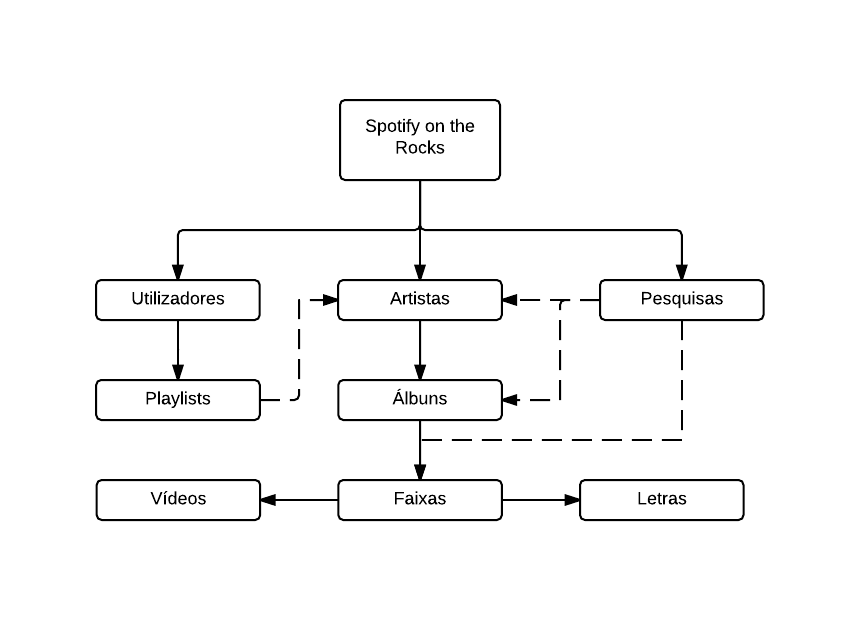
\includegraphics[width=0.5\textwidth]{concept_model}
    \caption{Modelo conceptual da aplicação}
    \label{fig:concept}
\end{figure}

As entidades são normalizadas após obtenção de informação de forma a a haver apenas três tipos de entidades base: Artistas, Álbuns e Faixas. Estas entidades definem a base dos compostos de informação presentes na aplicação e são expandidos através através de serviços externos de modo a complementar a informação, por exemplo: Vídeos oficiais ou de fãs ou letras das faixas em análise. Estas entidades são também a base para construções compostas como as \textit{Playlists} (listas de
reprodução) que, no caso de o Utilizador se encontrar devidamente autenticado com uma conta válida do Spotify, podem ser guardadas e experimentadas na plataforma músical. \\

\subsection{Diagrama de fluxo de dados da aplicação}

A figura~\ref{fig:flow} representa o processo de pesquisa da aplicação, após input do utilizador, na \textbf{API} do \textit{Spotify}, identificando as entidades presentes no resultado, convergendo-os para o motor da aplicação responsável pelo processamento e extensão da informação.
Para os resultados obtidos na construção (\textit{cocktail}) são efetuados posteriormente pedidos
a outros serviços, como por exemplo: \textit{SongMeanings} ou \textit{LyricFind} através das \textbf{APIs} disponíveis no \textit{The Echo Nest}, videoclips no \textit{Youtube}, ou informação adicional sobre a obra ou sobre o artista. \\
São também processados neste passo todas as métricas que aumentam o valor da informação obtida.

\begin{figure*}[hb]
    \centering
    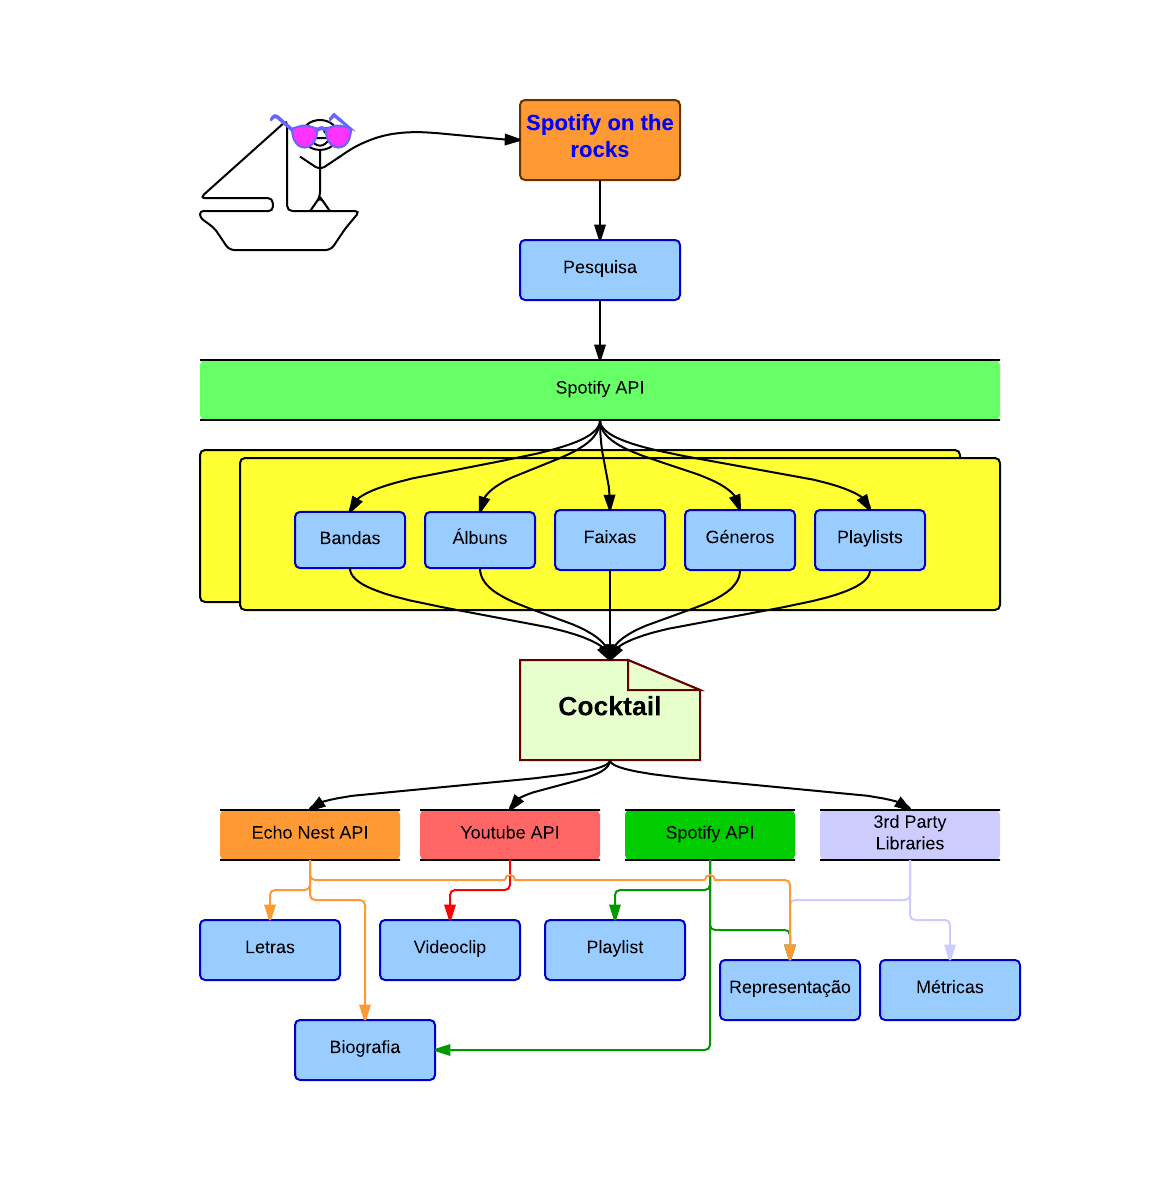
\includegraphics[width=\textwidth]{flow}
    \caption{Diagrama de fluxo de dados}
    \label{fig:flow}
\end{figure*}

\clearpage

%------------------------------------------------

\section{Tarefas de pesquisa}\label{sec:searches}

Com a aplicação anteriormente descrita, pretendemos que seja possível efetuar vários
tipos de pesquisa/operações sobre os dados que vamos utilizar, tais como:
\begin{compactitem}
  \item Procurar músicas por título, artista, álbum, género, país, ano ou uma combinação
    de qualquer destes campos, por exemplos:
    \begin{compactitem}
      \item procurar uma música do género Blues, cujo artista seja da Inglaterra;
      \item procurar uma música que seja um trabalho conjunto de 2 artistas;
    \end{compactitem}

  \item Obter uma lista de músicas através de combinações de pesquisas, podendo com
    isto criar uma playlist, se o utilizador estiver autenticado, como por exemplo:
    \begin{compactitem}
      \item uma playlist com 10 músicas dos Metallica e dos Muse;
      \item uma playlist com músicas portuguesas, ou com músicas portuguesas e
        brasileiras
    \end{compactitem}

  \item Utilizar a informação de uma música para obter a letra (\textit{lyrics}) a
    esta associada, através do \textit{SongMeanings}. Para além disso, podemos
    apresentar as discussões feitas acerca do significado dessa mesma música, uma vez
    que é esse o principal objetivo do \textit{SongMeanings};
    \item Permitir ao utilizador a visualização do \textit{videoclip} da música por ele procurada, através da integração com \textit{Youtube};
  \item Tirar partido das playlists dos utilizadores, para ver quantos \textit{followers}
    o \textit{Spotify} tem, e representá-los geograficamente (por exemplo, através de
      um mapa ou de um gráfico)
  \item Obter, através de toda esta informação, uma representação gráfica de dados
    estatísticos, como por exemplo:
    \begin{compactitem}
      \item número de utilizadores portugueses registados no spotify
      \item músicas mais ouvidas ou que são mais vezes avançadas (\textit{skipped})
      \item género musical mais apreciado pelos utilizadores
      \item \textit{word counter} em pesquisas conjuntas, seja ao nível de faixa, álbum,
        descrição, etc
    \end{compactitem}
\end{compactitem}

Consideramos que estes cenários de utilização serão bastante úteis, uma vez que o
\textit{Spotify} não possibilita pesquisas num âmbito tão alargado.

%----------------------------------------------------------------------------------------
%	REFERENCE LIST
%----------------------------------------------------------------------------------------

%% auto bibliographic list
%\renewcommand{\bibname}{Referências}
% uses bibtex file
% \bibliographystyle{unsrt-pt}
\bibliography{references}
% format for PT/EN alpha/unsrt
%\bibliographystyle{alpha-pt}
%\bibliographystyle{alpha}
\bibliographystyle{unsrt}

%----------------------------------------------------------------------------------------

\end{document}
